\section{The model's own confidence does not reveal the errors}
\label{sec:detect}
If misreadings came with uncertainty, the detectors already used to flag hallucinations would find them. We test three signals from the reader's own samples on the 456 synthetic questions shared with the proxy: disagreement among ten sampled answers, entropy of the sampled option distribution, and negative stated confidence \citep{selfcheckgpt,semantic-uncertainty,verbal-confidence}. None of them uses the answer key. For DeepSeek V4 Flash errors they reach AUROC 0.616 $[0.579, 0.656]$, 0.616 $[0.579, 0.656]$, and 0.617 $[0.558, 0.681]$ (Figure~\ref{fig:silent}a). On redefined common words they fall to 0.557, 0.557, and 0.463, against 0.60 to 0.72 on invented and usual-meaning terms (Appendix~\ref{app:signals-by-class}). The detectors fail precisely where local meaning is at stake. Our option-level entropy is narrower than semantic entropy over free-form answers \citep{semantic-entropy}, but the result agrees with the stability above. The small model's own uncertainty is no better. One minus its largest option probability reaches only 0.537 and 0.523 on redefined common words for the two readers.

Better calibration does not close the gap. Jev \citep{jev} is a decision model built to report calibrated confidence. Its confidence ranks its own errors without a definition with AUROC 0.643 on synthetic, 0.660 on Reddit, and 0.636 on CUAD questions, and with a model-drafted local gloss added, with 0.815, 0.790, and 0.868 (Figure~\ref{fig:silent}b). The same confidence channel works once the local meaning is present, an observation consistent with a limitation of information rather than calibration. A model cannot flag a meaning it does not know has changed, so confidence thresholds, abstention rules, and sample agreement tuned on ordinary errors pass these answers.

\begin{figure}[t]
\centering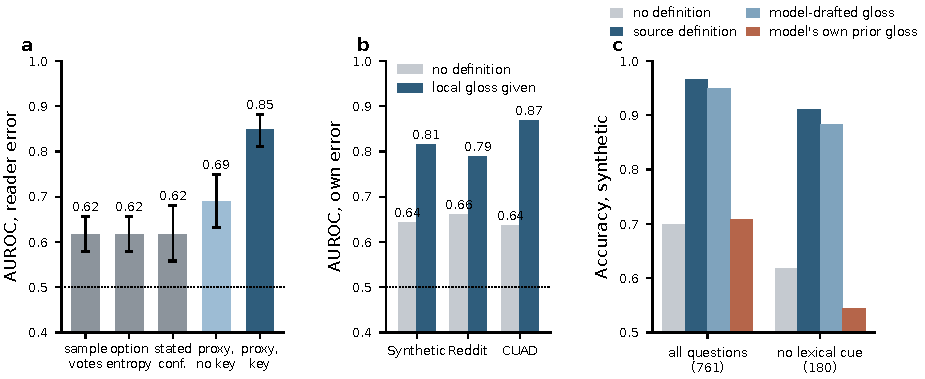
\includegraphics[width=\linewidth]{figs/silent_repair.pdf}
\caption{(a) AUROC for ranking DeepSeek V4 Flash errors on 456 synthetic questions, with 95\% intervals from resampling terms. Gray bars are key-free signals from the reader's ten samples and stated confidence. The light bar is the key-free uncertainty of the 7B proxy (one minus its largest option probability). The dark bar is the proxy score $R$, which checks the proxy against the source-implied answer. The dotted line marks chance. (b) Jev's native confidence as a detector of its own errors, without a definition and with a model-drafted local gloss. (c) DeepSeek V4 Flash accuracy on synthetic questions under four conditions: no definition, the source definition, a model-drafted gloss, and the model's own gloss of the term written under a domain prompt. The right group keeps only questions where no option is singled out by word overlap with any of the three texts.}
\label{fig:silent}
\end{figure}
